\documentclass[twocolumn, 10pt, a4paper]{memoir}

% standard packages
\usepackage{titlesec, blindtext, color}                                  % standard packages
\usepackage[usenames,dvipsnames,svgnames,table]{xcolor} % extra colors
\usepackage{graphicx}    
\usepackage{amsmath}                                                   % figures
%\usepackage{natbib}                                                          % bibliography
\usepackage{apacite}
\usepackage[english]{babel}
\usepackage{multirow}                                              % correct hyphenation (afbreekstreepjes)
\usepackage{booktabs}                                                     % for midrule in tables
\usepackage{array}
\newcolumntype{P}[1]{>{\raggedright\arraybackslash}p{#1}}
\usepackage[modulo, switch]{lineno}   % use for linenumbers at the sides
% PAGE MARGINS
\usepackage[top=2.5cm, bottom=2.5cm, left=2cm, right=2cm]{geometry}

% FONT
\usepackage[lf]{berenis}
\renewcommand*\familydefault{\sfdefault}
\usepackage[T1]{fontenc}
% for other fonts, and how to install them, see the LaTeX Font Catalogue:
% http://www.tug.dk/FontCatalogue/

% LINE SPACE
\linespread{1.2}                          % more space between lines
\setlength{\parindent}{7mm}       % indenting first line paragraph
\setlength{\columnsep}{7mm} % space between columns
\linenumbers
% TABLE OF CONTENTS
% for subsubsection headers (e.g. 2.1.3), write subsubsection
% for subsection headers (e.g. 2.1), write subsection
\setsecnumdepth{subsection}        % in text
\settocdepth{subsubsection}              % in table of contents
\renewcommand{\cftdot}{}          % for no dots in table of contents
\cleardoublepage

% HYPHENATION (afbreekstreepjes)
% set words that are not abbreviated correctly (expand list when necessary)
\hyphenation{catch-ment areas a-na-lyse}

\graphicspath{ {./images/} }
%%%%%%%%%%%%%%%%%%%%%%%%%%%%%%%%%
% headers: page numbers and running titles
%%%%%%%%%%%%%%%%%%%%%%%%%%%%%%%%%

\makepagestyle{ruled}
\makeevenfoot{ruled}{}{}{}  % empty footer
\makeoddfoot{ruled}{}{}{}   % empty footer

% header left page (text on left, middle and right slot empty)
\makeevenhead{ruled}{\textcolor{gray}
	{\makebox[6mm][l]{\thepage} $|$ \hspace{3mm} \leftmark}}{}{}

% header right page  (text on right, middle and left slot empty)
\makeoddhead{ruled}{}{}{\textcolor{gray}
	{\rightmark \hspace{3mm} $|$ \makebox[6mm][r]{\thepage}}}

% first page of chapter
\titleformat{\chapter}[hang]{\vspace{-34mm}\huge}{\thechapter\hspace{20pt}\textcolor{gray}{|}\hspace{20pt}}{0pt}{\huge}
\aliaspagestyle{chapter}{chapterheader} % for no page numbers on first chapter page


%%%%%%%%%%%%%%%%%%%%%%%%%%%%%%%%%
% for background figure first page
%%%%%%%%%%%%%%%%%%%%%%%%%%%%%%%%%

\usepackage{eso-pic}
\newcommand\BackgroundPic{%
	\put(0,0){%
		\parbox[b][\paperheight]{\paperwidth}{\vfill
			\centering
			\includegraphics[width=\paperwidth,height=\paperheight,keepaspectratio]{figs/backgroundfigure.jpg}%
			\vfill
}}}



%%%%%%%%%%%%%%%%%%%%%%%%%%%%%%%%%
%%%%%%%%%%%%%%%%%%%%%%%%%%%%%%%%%
% START
%%%%%%%%%%%%%%%%%%%%%%%%%%%%%%%%%
%%%%%%%%%%%%%%%%%%%%%%%%%%%%%%%%%

\begin{document}
	
	\thispagestyle{empty}                    % otherwise it gives page number on first page
	\pagestyle{empty}
	\frontmatter
	\firmlists 
	
	\section{Intro for Thesisring}
	Hi everyone, a late submmission to the thesisring but I just finished my Data section and saw that there was still a free spot on the submission list ;) 
	\newline
	I tried to write my data section as concise as possible: writing it in such a way that there is the minimal amount of required information, but without missing parts. The thing that I would be interested in most is:
	\begin{enumerate}
		\item Do you agree with this concise writing style?
		\item Is there any important information missing from the mentioned datasets?
		\item Do the figures help to give a bit of insight into the data and if not, do you have any suggestions on what could possibly be added in terms of figures?
	\end{enumerate} 
	It is not a very long datasection so it should not take too much time, but I'd still like some feedback wherever possible :)
	\newline
	Thank you! 
	%%%%%%%%%%%%
	% FIELD SITE AND DATA
	%%%%%%%%%%%%
	\openany
	\chapter{Data}\vspace{-6mm}\label{ch: field}
	In this study, two types of data are used: CML signal data which is used as input to the model, and precipitation observations as reference to evaluate the model. Both types of data will be elaborated upon in this section.
	
	\section{Commercial Microwave Link data} \label{sec: CML data}
	The CML data used in this research is the same as used in previous research \shortcite{Overeem2016}.
	The CML data is required from NOKIA microwave links, operated by T-Mobile. The dataset spans from January 14 2011 until June 30 2013. The dataset consists of  3101 links, but as shown before \shortcite{Overeem2016}, not all of these links are useful or continuously available. The total number of actual links used will therefore be lower, depending on the quality. Received Signal Level (RSL) in decibel-milliwatts (dBm) is stored at 15-minute intervals, at which the minimum and maximum signal level over the time period are stored. The power resolution of this data is 1 dB. 
	
	\begin{figure}[h]
		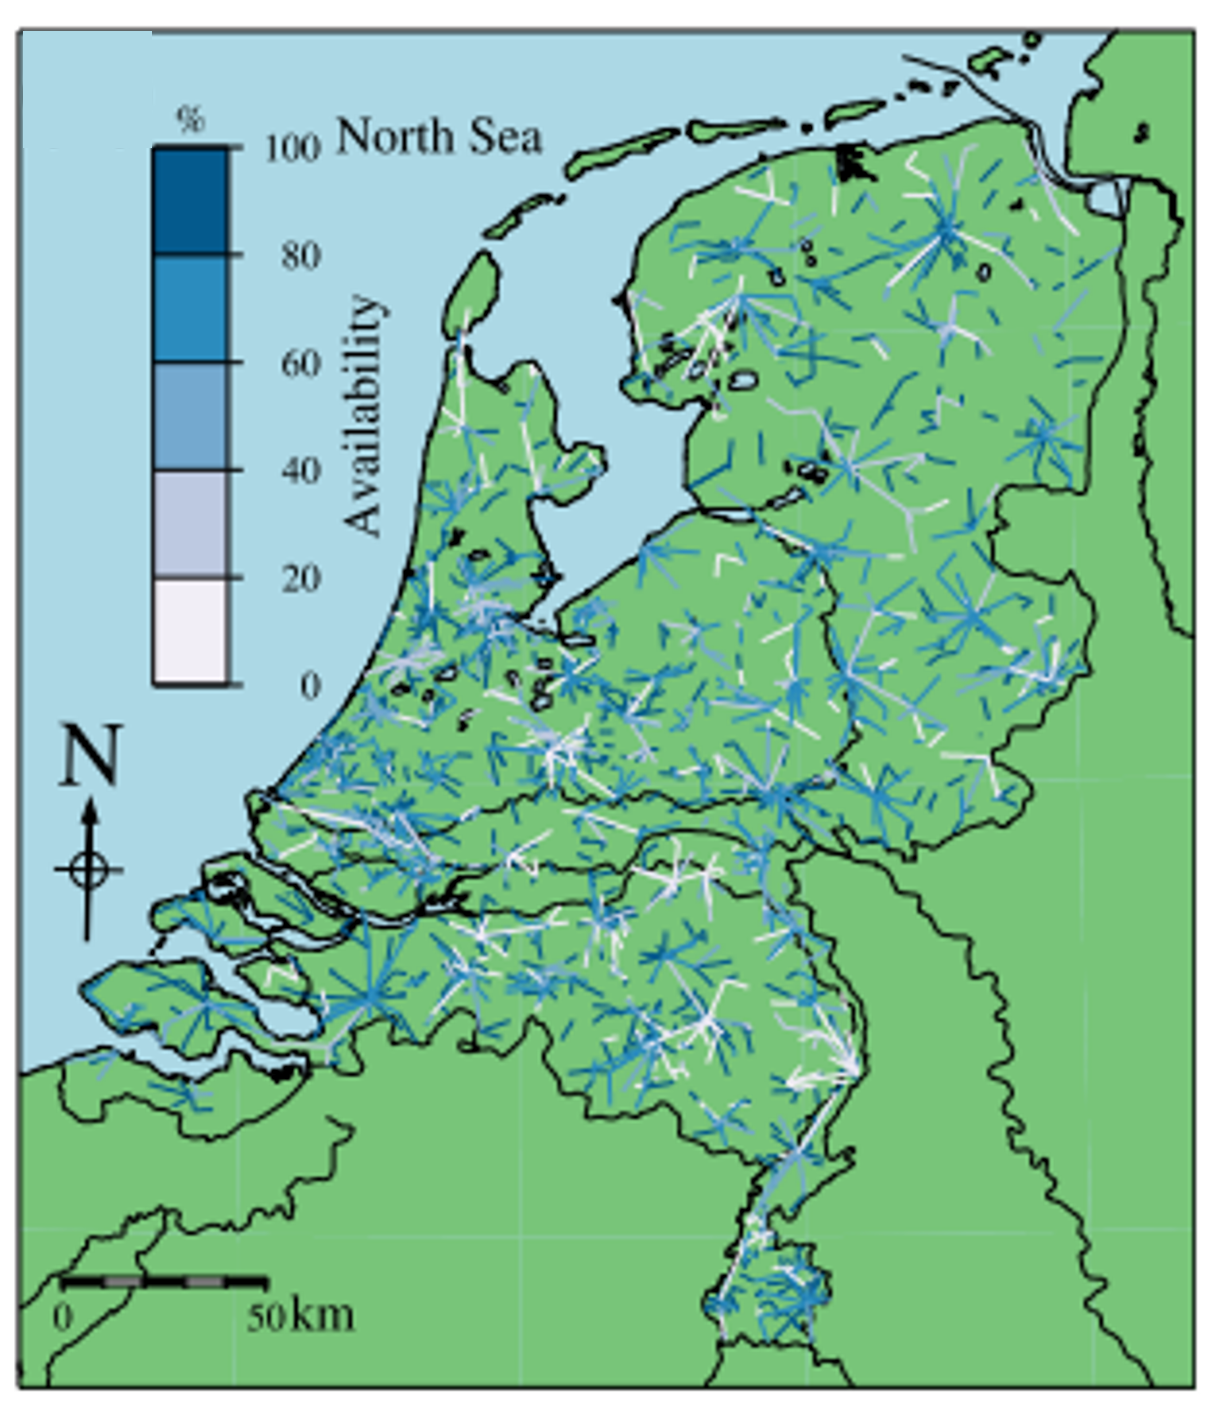
\includegraphics[height= 9cm]{Dutch_CML_network}
		\caption{Used CML network in the Netherlands. Retrieved from \protect\citeA{Overeem2016}}
		\label{fig: cmlnetworkmaps}	
	\end{figure}
	
	\begin{figure}[h]
		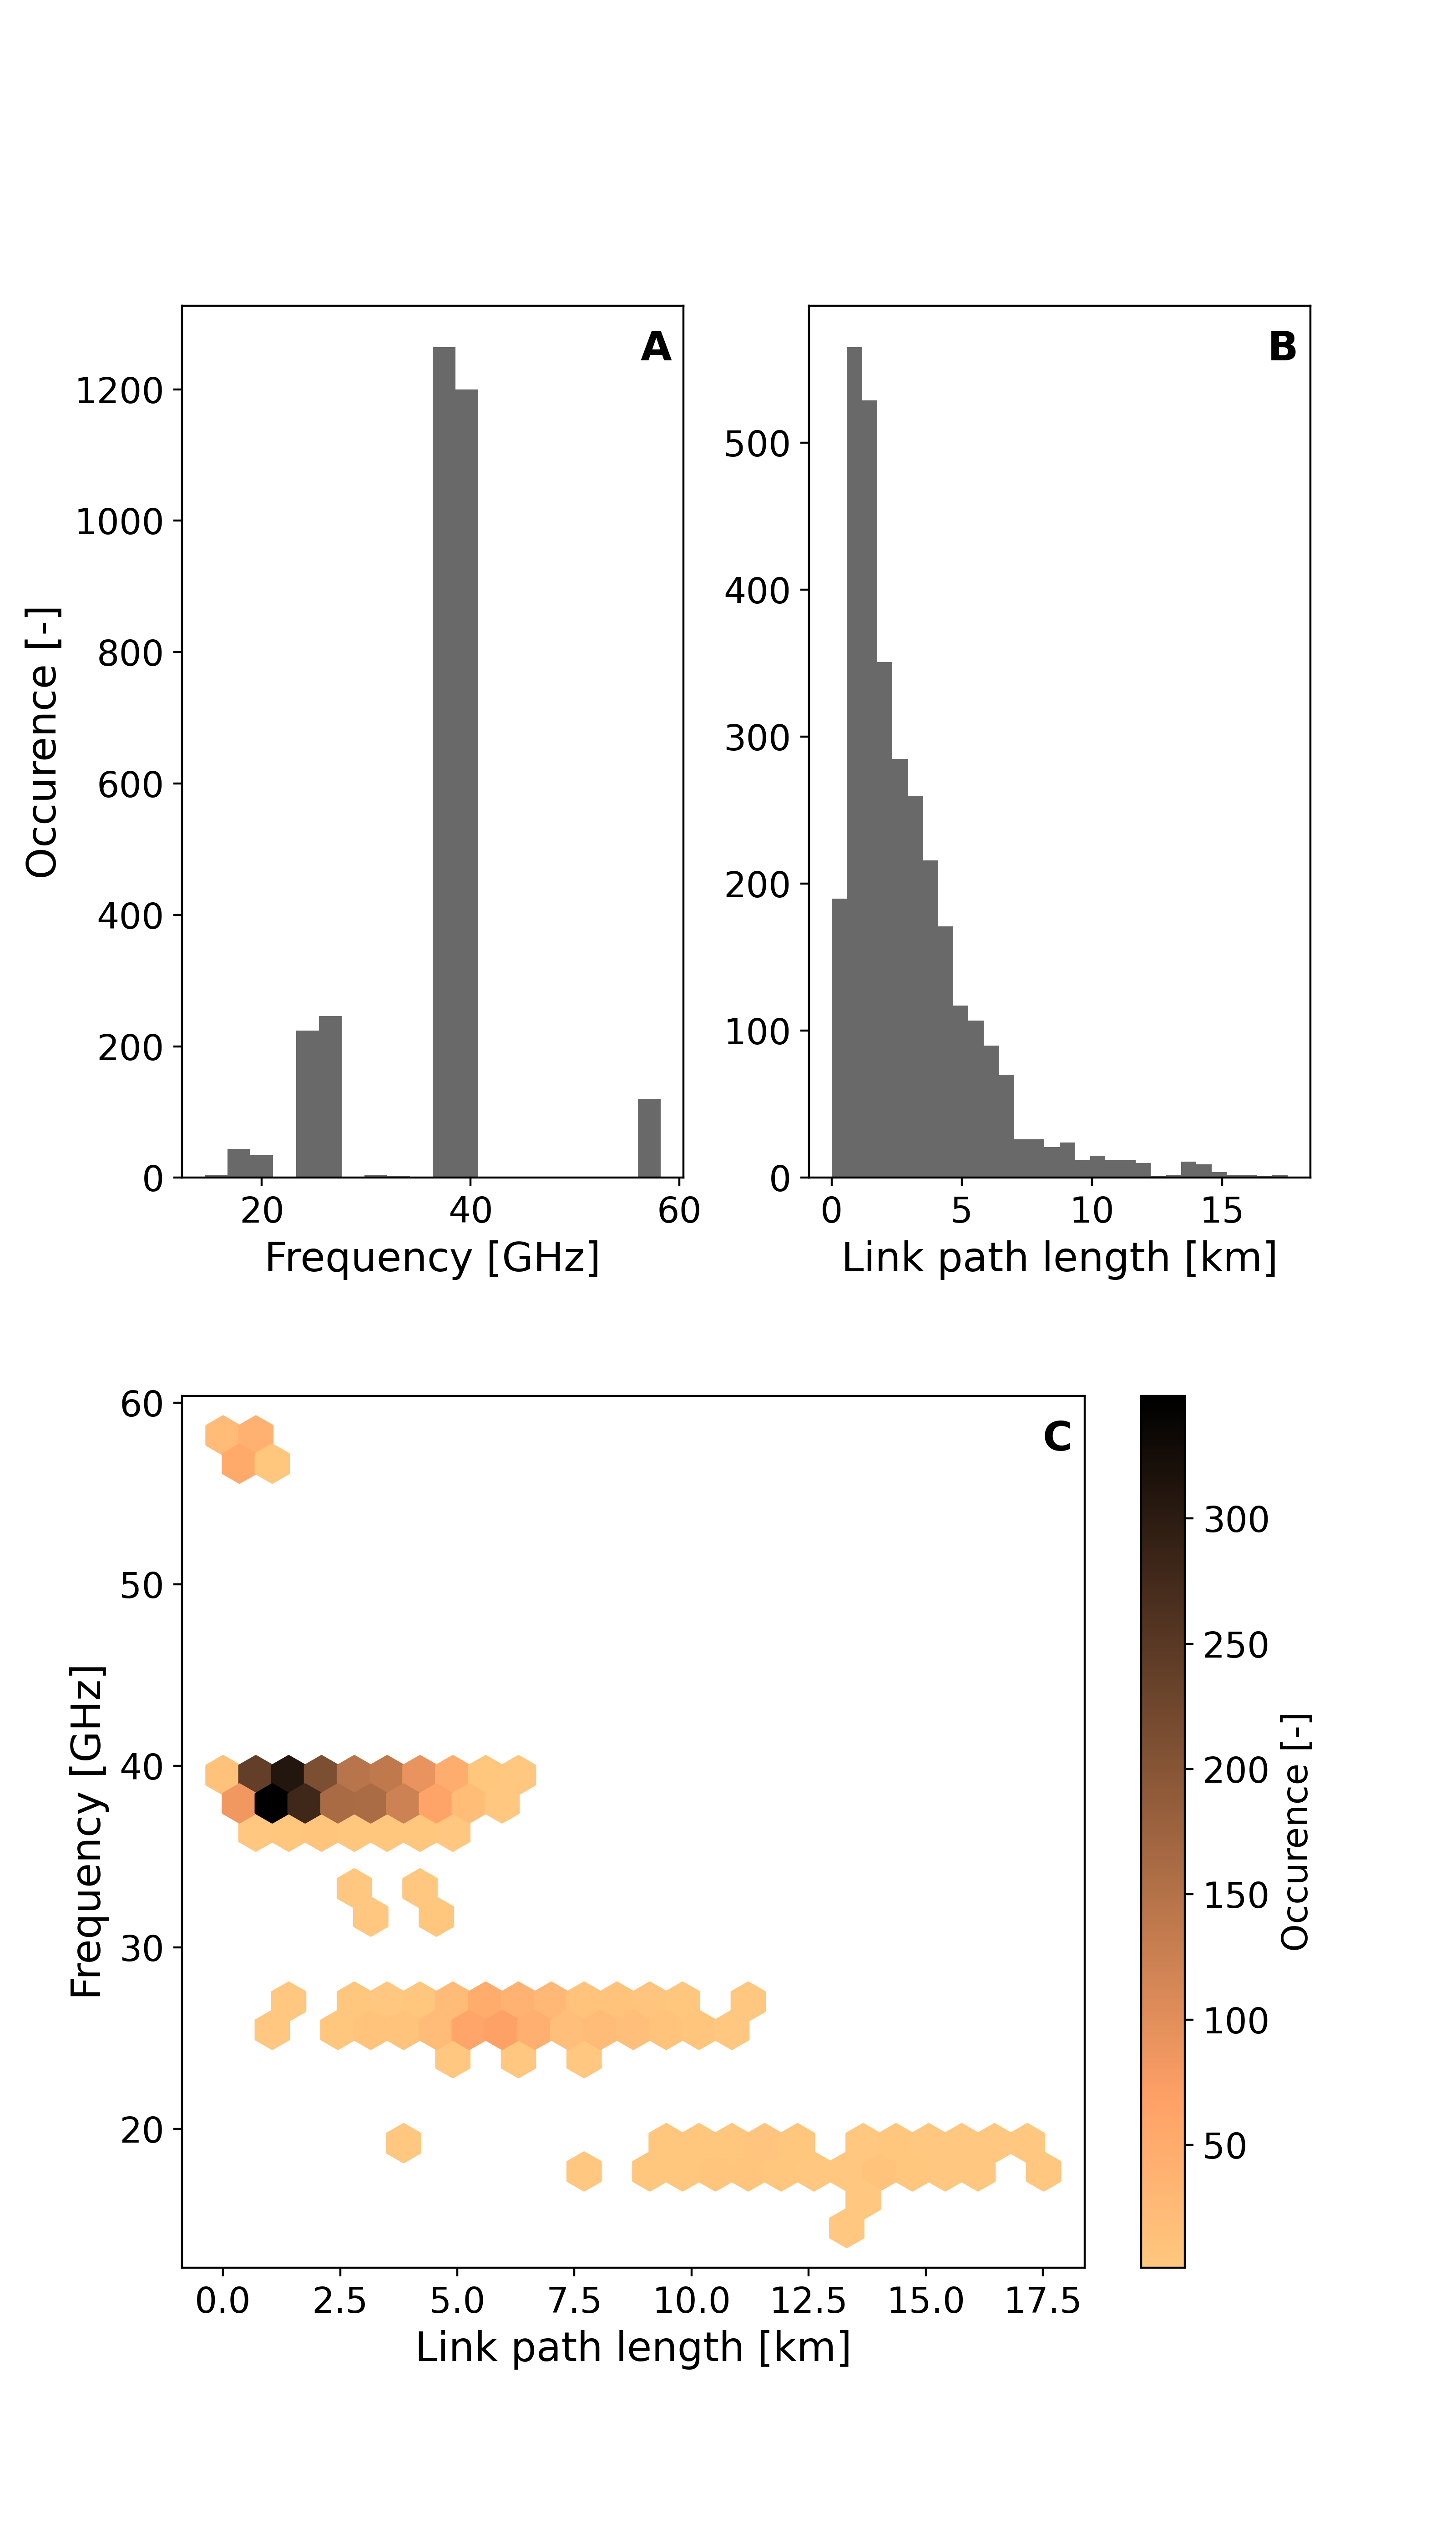
\includegraphics[width=10cm]{val_freq_dist}
		\caption{Frequency and distance distributions for the CML data. Figures apply to the final independent test set covering half of 2013}
		\label{fig: CML validation}
	\end{figure}
	
	Apart from the dynamic time signal data, static metadata is included as well. This includes coordinates of the start and end point of the link, distance between these points and frequency per link. Figure \ref{fig: cmlnetworkmaps} shows the distribution of the links throughout the Netherlands. As the frequency at which the links operates and the distance the link covers determine the baseline for the link's signal, their respective distributions can be found in Figure~\ref{fig: CML validation}. The spikes in the frequency distributions indicate that the links roughly operate at 4 different frequencies. The distance distributions shows that although most links operate at quite short distances (<2 km), there are still links included in the data set that cover over 5 or even 10 km.
	
	
	\section{Reference precipitation data} \label{sec: Ref prec data}
	The precipitation observations are taken from the gauge-adjusted radar rainfall product (freely available as "Radar precipitation climatology" via http://climte4impact.eu) with a resolution of 0.9 km\textsuperscript{2}. The radarmeasurements are adjusted with the use of both automated and manual rain gauge networks operated by the Royal Netherlands Meteorological Institute (KNMI). The gauge-adjusted radar observations are at a 5-min temporal resolution. To match the 15-min intervals from the CML data, the precipitation data is summed to 15-min intervals. 
	
	\openany
	\renewcommand{\bibname}{Bibliography}
	\bibliographystyle{myapacite}
	\bibliography{Thesis_Ludo}
	
	% to add items to the bibliography:
	% option 1. open "references_thesis.bib" in JabRef (free downloadable), enter more papers
	% option 2. open "references_thesis.bib" in NotePad, go to Google Scholar, find paper, click "cite", click "import into BiBTeX", copy text into NotePad
	
	

	
	
	%%%%%%%%%%%%%%%%%%%%%%%%%%%%%%%%%
	% END
	%%%%%%%%%%%%%%%%%%%%%%%%%%%%%%%%%
	
	
\end{document}